\section{Finite-sample neural growth: realized effects and failed extensions}
\label{sec:experiments}

The preceding statements concern population risks and prescribed operations.
We therefore conducted actual neural training experiments in which the controller
observes only sampled labels. These experiments test three different questions:
can sampled operational statistics recover the useful split direction; does that
initial advantage survive optimization; and can an empirical gate avoid
unnecessary growth? A separate exploration tests a conditional-information
operation score under ordinary random neural initialization. None of these
experiments identifies representation states with neurons.

\subsection{Parameterized system and controller information}

The trained predictor is
\[
 p_\theta(x)=\operatorname{sigmoid}\left(c+\sum_{j=1}^k
 a_j\tanh(b_j+w_j^\top x)\right).
\]
The trainable objects are actual hidden units with input weights $w_j$, biases
$b_j$, output coefficients $a_j$, and a common intercept $c$. A split duplicates
unit $j$, halves its output coefficient, and replaces its two input weights by
$w_j+\varepsilon v$ and $w_j-\varepsilon v$. All input weights, hidden biases,
output coefficients, and the intercept are subsequently trained without a tying
constraint. At $\varepsilon=0$ this operation preserves the predictor exactly;
for positive $\varepsilon$ it is a controlled perturbation, followed by a real
change in parameter count. Retraining may change predictions at every old input.
It need not create a nested discrete partition.

For the theory-linked experiment, the learned direction is the smallest
eigenvector of
\[
 \widehat S_j=\frac1n\sum_{i=1}^n
 [p_\theta(x_i)-y_i]a_j\tanh''(b_j+w_j^\top x_i)x_ix_i^\top.
\]
This is an operation-specific curvature statistic, not marginal activation
entropy. Its implementation observes input coordinates, residuals, and the
current parameters. It receives neither the population conditional label
probabilities nor a supplied signal direction. The random-direction control
uses a normalized standard Gaussian vector. A separately labelled population
curvature oracle computes $S_j$ from the complete known synthetic population;
it is a diagnostic and does not enter either learned controller. At the
constant start, an activation-only scalar statistic has no directional
information; the random control is the deliberately uninformative directional
comparison, rather than an invented entropy optimizer.

\subsection{The controlled bridge and its validity tests}

We use five regimes. The four-state regime is uniform on
$\{\pm e_1,\pm e_2\}$ with conditional label probabilities $0.65$ on the first
axis and $0.35$ on the second. The width-one initial parameters are
$w=0$, $b=0.5$, $a=1$, and $c=-\tanh(0.5)$, so the initial prediction is $1/2$.
The rotated regime is uniform on the sixteen points $\{\pm Qe_j:1\leq j\leq8\}$,
where each repetition draws a new orthogonal matrix by QR factorization of a
Gaussian matrix. Label probabilities are $0.65$ and $0.35$ on its first two
axes and $0.5$ on the remaining axes. Thus the controller must discover the
input geometry amid six irrelevant axes. The sample-pretrained regime uses
this rotated task but first trains the width-one model for 100 updates from
the special initialization. The random-start regime instead initializes all
width-one weights randomly and trains for 100 updates. The no-signal regime
uses the rotated inputs with every label probability equal to $0.5$.
These tests distinguish a deliberately designed stationary start from a
checkpoint obtained through ordinary sample training.

Each regime uses $n\in\{256,1024\}$ IID training examples and an independent
validation sample of the same size. A sample contains ordinary Bernoulli labels;
there is no importance sampling or enumerated-label training. The split uses
$\varepsilon=0.6$. Each branch receives either $T=30$ or $T=300$ full-batch Adam
updates with learning rate $0.02$, standard momentum coefficients $0.9,0.999$,
and numerical denominator constant $10^{-8}$. Optimizer moments are reset at
each branch, including the continuation control. The shared pre-split checkpoint
is identical for the spectral, random, and oracle branches. All parameters are
untied and trained after the split. The two budgets are separate runs, not
selected stopping times. For numerical stability, the code clips
predicted probabilities to $[10^{-9},1-10^{-9}]$ for evaluation; the
maximum absolute logit across all saved fitted bridge branches is 6.852,
well inside the clipping threshold of 20.723. Thus that clip does not
alter their reported population losses.

There are 64 independent repetitions per regime, sample size, and budget,
using seeds 27100 through 27163. This gives 1280 completed training configurations.
Shared random seeds make within-configuration method comparisons paired;
confidence intervals never treat the methods or input points as independent
replicates. We report Student-$t$ intervals across the 64 seed-level paired
risk differences. They are descriptive intervals for these synthetic regimes,
without a multiple-comparison claim. Risk evaluation integrates both the finite
input distribution and the conditional label law exactly. This exact evaluation
is distinct from the finite-sample learning that produced each network.

The autonomous variant fits both the grown model and a width-one continuation.
On the disjoint validation sample it computes their paired per-example log-loss
improvements $D_i$, accepting growth only if
$\overline D>1.96\,s_D/\sqrt n$. Otherwise it keeps the continuation.
This fixed normal-approximation rule is a heuristic gate, not a theorem-level
finite-sample confidence guarantee. Both spectral and random proposals use the
same rule and validation sample. The gate therefore does not silently borrow
population information, but it does pay for two fitted branches and additional
labelled validation data. Its comparison with an ungated continuation does not
by itself isolate the value of the spectral principle.

\subsection{Capacity, compute, data, and implementation controls}

A width-$k$ model in dimension $d$ has $k(d+2)+1$ trainable parameters. The bridge
therefore grows from $d+3$ to $2d+5$ parameters. Spectral and random growth have
identical final architecture, shared initialization, training data, update count,
and optimizer. Their additional controller costs differ: forming the spectral
matrix costs $O(nd^2)$ arithmetic and its eigendecomposition costs $O(d^3)$;
random direction generation costs $O(d)$. These overheads are explicitly
additional, although small in these low-dimensional experiments.

We also train fixed width-two networks from standard random initialization.
One comparison matches the number of optimization updates, including any
width-one pretraining. A second matches the approximate number of
parameter-example updates: after $P$ pretraining steps and $T$ growth steps,
the fixed model receives
\[
 T+\left\lfloor\frac{P(d+3)}{2d+5}\right\rfloor
\]
updates. This is an operation-count proxy, not a claim of identical measured
FLOPs, optimizer cost, or wall time. $P=0$ for the prescribed stationary starts
and $P=100$ for the two pretrained regimes. We do not call equal updates and
equal compute the same comparison. All methods use the same training examples;
only gated decisions consume the separate validation labels. Raw records retain
these resource formulas, controller costs, selected directions, split matrices,
immediate and post-training risks, validation events, prediction changes,
parameter displacements, and fitted network parameters.

The reported parameter counts describe individual predictors, not total live
process memory. A gate retains a continuation and a growth candidate, together
with optimizer state during fitting; its peak memory and branch-training cost
exceed the final predictor size. The implementation additionally fits every
comparison and oracle for measurement. Those research costs cannot be credited
as free online adaptation. The entire 1280-configuration bridge run took
85.53 seconds on the local CPU environment; this aggregate wall time is not a
per-method runtime comparison.

Independent implementation checks compare analytic gradients against central
finite differences (maximum absolute error $8.16\times10^{-11}$), verify exact
function preservation at zero split displacement, and compare the actual
small-displacement risk change with the derived quadratic term. At
$\varepsilon=10^{-4}$ their ratio is $1.000000199$. These checks support the
implementation; they do not replace the mathematical proofs.

\begin{table}[tb]
\centering\footnotesize\setlength{\tabcolsep}{4pt}
\caption{Actual finite-sample neural training at $n=1024$. Entries are exact population log loss after fitting; $\Delta$ is the paired spectral-minus-random mean with a 95\% Student-$t$ interval half-width across 64 independent seeds. $T$ is the post-growth update budget. Fixed width uses the approximate parameter-update budget described in the text. Lower is better.}
\label{tab:neural-results}
\begin{tabular}{@{}llrrrrr@{}}
\toprule
Regime & $T$ & Spectral & Random & Fixed 2 & Continue 1 & $\Delta\pm$ half-width\\
\midrule
Four states & 30 & 0.65606 & 0.66809 & 0.68782 & 0.69323 & $-0.012033 \pm 0.003104$ \\
Four states & 300 & 0.64928 & 0.64928 & 0.65256 & 0.68002 & $-0.000002 \pm 0.000003$ \\
Rotated 8D & 30 & 0.69175 & 0.69458 & 0.69526 & 0.69744 & $-0.002827 \pm 0.000588$ \\
Rotated 8D & 300 & 0.68955 & 0.68971 & 0.69159 & 0.69488 & $-0.000162 \pm 0.000251$ \\
Random start & 30 & 0.69473 & 0.69450 & 0.69352 & 0.69450 & $+0.000236 \pm 0.000180$ \\
Random start & 300 & 0.69373 & 0.69371 & 0.69124 & 0.69421 & $+0.000019 \pm 0.000609$ \\
No signal & 30 & 0.69866 & 0.69797 & 0.69640 & 0.69770 & $+0.000691 \pm 0.000179$ \\
No signal & 300 & 0.70064 & 0.70068 & 0.70008 & 0.69805 & $-0.000046 \pm 0.000064$ \\
\bottomrule
\end{tabular}
\end{table}


\begin{figure}[tb]
 \centering
 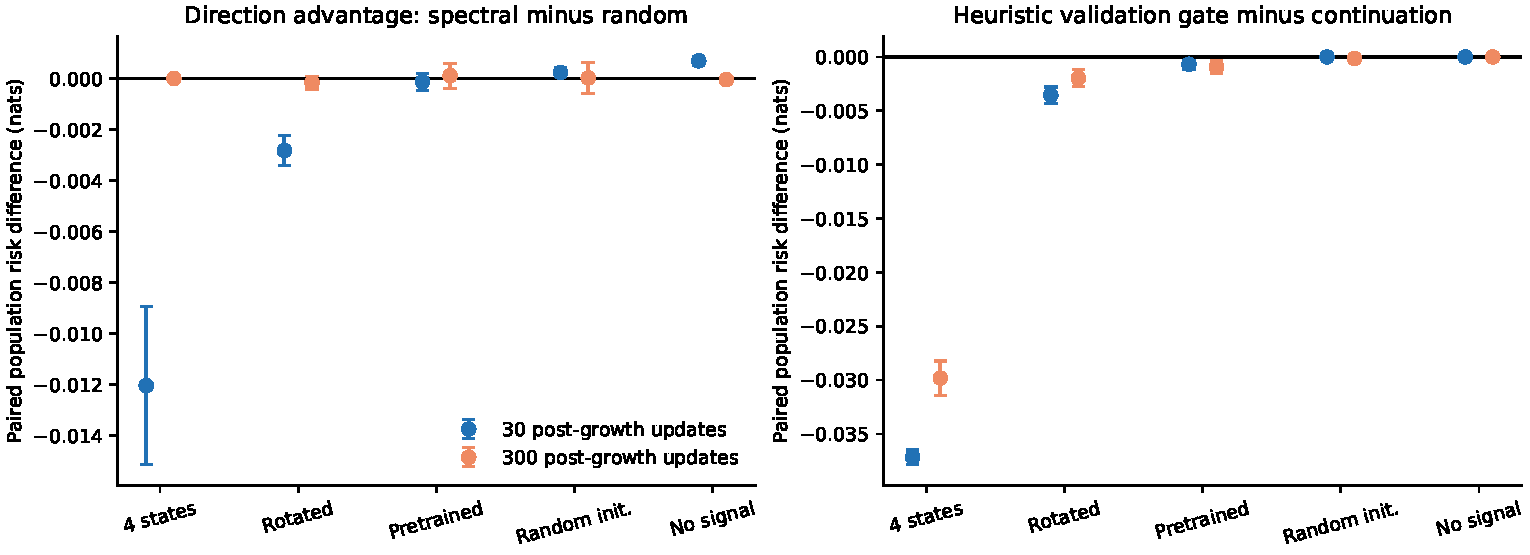
\includegraphics[width=\textwidth]{../figures/learning_curvature_differences.pdf}
 \caption{Measured neural training results at $n=1024$. Left: spectral minus
 random split risk at identical architecture and training budgets. Right: the
 heuristic validation-gated spectral model minus width-one continuation; this
 latter comparison additionally uses validation labels and branch-training
 compute. Points average 64 paired repetitions; bars are 95\% Student-$t$
 intervals. Every risk is evaluated exactly on the finite population after
 fitting from IID labelled samples. Negative values favor the spectral or
 gated method.}
 \label{fig:bridge-differences}
\end{figure}

\subsection{What the bridge established, and where it failed}

At the prescribed four-state start the learned spectral direction selects the
correct axis in all 64 repetitions at both sample sizes. Its immediate
population loss reduction is $0.00759820$ nats; random directions have negative
mean reductions, i.e. they initially increase the loss. At $n=1024$ and 30
updates, spectral growth has mean risk $0.656061$, compared with $0.668094$ for
random growth. Because those branches share the same capacity, data, training
budget, and initial checkpoint, this is evidence for the operational direction
choice in the designed regime, subject to its extra matrix-estimation cost.
After 300 updates their risks are $0.649278$ and $0.649280$; the directional
advantage has essentially disappeared. Thus the local geometric advantage is
not a persistent representational advantage when later optimization can
reorganize both models.

On the rotated task, the spectral proposal immediately improves population
loss in 44 of 64 repetitions at $n=256$ and 61 of 64 at $n=1024$. Its immediate
mean gain rises from $0.001245$ to $0.001795$ nats, compared with $0.001900$ for
the population curvature oracle. At $n=1024$ its 30-update advantage over random
splitting is $0.002827$ nats; it shrinks to $0.000162$ after 300 updates.
At $n=256$, longer retraining instead overfits: spectral population risk grows
from $0.709556$ after 30 updates to $0.722064$ after 300, both above the
constant-predictor risk $\log 2$. This is not hidden by reporting only ratios or
training accuracy.

The sample-pretrained and random-start tests are essential limitations.
After ordinary width-one sample training, the selected spectral direction is
no longer reliably aligned with the designed signal. In the random-start
regime at $n=1024$, its 30-update risk is slightly higher than random growth
($0.694734$ versus $0.694498$). At 300 updates there is no resolved difference.
The experiment therefore does not establish a generally useful growth rule at
arbitrary trained checkpoints. Moreover, finite-sample training can move along
initially neutral parameter directions and escape the particular population
local minimum: width-one continuation is not required to remain constant.
The observed continuation improvements do not contradict a local population
statement at a specified parameter point.

Every forced spectral split in the no-signal task increases the immediate
population loss. At $n=1024$ the validation gate accepts zero of 64 spectral
proposals at both budgets; at $n=256$ it accepts one of 64 at each budget.
On the rotated $n=256$, 300-update condition it rejects all 64 proposals,
preventing selection of the heavily overfit grown networks. Rejection is
relative to a fitted continuation, which may itself overfit; the gate does not
recover the unknown Bayes predictor or prove universally safe adaptation.
These are empirical gate diagnostics, not an automatic conversion of the
curvature theorem into a finite-sample acceptance guarantee.

\subsection{Independent random-initialization information-score probe}
\label{sec:information-probe}

Before choosing the theory-linked experiment, an independent investigation
implemented actual width-two to width-three growth on continuous Gaussian
inputs. It initially used the conditional label information of the
\emph{antisymmetric child-activation contrast}
$\tanh(a+\delta u)-\tanh(a-\delta u)$, where
$a=b_j+w_j^\top x$ and $u=v^\top x$.
Independent adversarial review identified a material limitation: this feature
contrast is not the symmetric predictor deformation caused by the prescribed
initial split. Its negative result cannot establish failure of an
operation-aligned information score. We retain all original runs and add a
fresh-seed ablation with the exact initial logit deformation
\[
 Z_v(x)=a_j\left\{\frac{\tanh(a+\delta u)+\tanh(a-\delta u)}2-\tanh(a)\right\}.
\]
The corrected feature definition was fixed before drawing its new seeds.

Each candidate is scored by the plug-in conditional mutual information between
its three-bin feature and the binary target, conditional on a three-quantile-bin
current prediction. The aligned feature uses three empirical quantile bins.
The original antisymmetric feature instead uses the fixed thresholds
$-0.08,0.08$; its marginal entropy is retained as a separate baseline. Thus
``entropy'' here refers to that specified three-state activation-contrast
histogram, not differential entropy. The conditioning variable is a lossy
quantization of the current prediction, not the full neural representation.
Consequently neither score is automatically the recoverable predictive
information of the full model, and neither provides a Bayes-refitting guarantee
for the trained network.

For each run, 512 examples train the network, 512 disjoint labelled examples
score candidate operations, and 8192 independent inputs evaluate it using the
known teacher label probabilities. This evaluation integrates the conditional
Bernoulli label law exactly but only Monte Carlo averages the continuous input
distribution; it is not an exact population calculation. Population probabilities
are never passed to learned selectors. The deliberately optimistic evaluation
oracle chooses the candidate with minimum loss on those same 8192 evaluation
inputs, and is labelled as an evaluation oracle rather than an implementable
controller or an exact population optimizer.

All three tasks use $X\sim N(0,I_3)$ and
$P(Y=1\mid X)=0.05+0.90\operatorname{sigmoid}(g(X))$.
The linear-null task has $g(x)=2x_1$. The localized task has
$g(x)=1.5x_1+4\tanh(2x_2+1)\tanh(2x_3-1)$.
The teacher task uses four tanh units with fixed weights, biases, and output
coefficients specified exactly in the released code. Width-two students start
randomly and receive 300 full-batch Adam updates with learning rate $0.025$.
Each of the two units has four independently drawn Gaussian split directions,
normalized to unit length, for eight candidate operations. The perturbation
scale is $\delta=0.25$ and each candidate then receives 150 updates of all
parameters. Random choice, the two information scores, and marginal entropy
select among the same candidates before retraining. A separately labelled
trained-validation control trains all eight candidates and selects by score-set
log loss. It has an eightfold candidate-fitting cost; that benefit cannot be
credited to a cheap information score. Width-two continuation and fixed
width-three controls receive the corresponding prescribed update budgets.
Information scoring uses 512 additional labelled score examples; random
selection does not use those labels, and the entropy proxy uses only score
inputs. Therefore any positive comparison with random selection would also
have to account for this extra supervised information. Here no resolved aligned
CMI advantage survives even with that access. The fixed-width approximate
compute comparator scales the width-two pretraining budget by $2/3$, explicitly a leading-width proxy rather than exact
parameter/FLOP matching.

The original four-seed pilot used 250 pretraining updates and is preserved;
subsequent exploratory and aligned runs use 300. Thus the pilot-to-expanded
comparison does not change only the repetition count. The 32-seed exploratory
run is also preserved, with seeds $17000,\ldots,17031$. The aligned ablation uses 32 new seeds
$41000,\ldots,41031$ after the audit-triggered definition change. No fresh evaluation
result was used to tune that feature definition, the bin count, the optimizer,
or the candidate perturbation. It remains a small synthetic mechanism study,
not a broad benchmark or a universal rejection of information-guided growth.

For complete specification, the teacher function is
$g(x)=\tanh(x^\top W+\beta^\top)\alpha$ with
\[
 W=\begin{pmatrix}
 1.8&-1.4&0.4&1.2\\
 0.4&1.8&-1.7&0.8\\
 -1.5&0.3&1.3&-1.2
 \end{pmatrix},\qquad
 \beta=(0.4,-0.5,0.2,1)^\top,\qquad
 \alpha=(2,-2,2,-1.5)^\top.
\]
Standard random initialization in both studies uses independent input weights
$N(0,0.8^2)$, hidden biases $N(0,0.1^2)$, output coefficients
$N(0,0.5^2)$, and intercept zero.

\begin{table}[tb]
\centering\footnotesize\setlength{\tabcolsep}{5pt}
\caption{Fresh-seed operation-aligned information-score ablation. Risks integrate the teacher label probability on 8192 held-out Gaussian inputs, and are averaged across 32 seeds. The last column gives aligned-CMI minus random-growth risk with a paired 95\% Student-$t$ interval half-width. Fixed width 3 uses the leading-width compute proxy; its initialization differs from the grown model.}
\label{tab:aligned-probe}
\begin{tabular}{@{}lrrrrr@{}}
\toprule
Task & Aligned CMI & Random & Entropy & Fixed 3 & Difference $\pm$ half-width\\
\midrule
teacher & 0.40350 & 0.40250 & 0.40364 & 0.40093 & $+0.00100 \pm 0.00159$ \\
localized & 0.51857 & 0.51594 & 0.49348 & 0.48874 & $+0.00263 \pm 0.00991$ \\
linear null & 0.53534 & 0.53601 & 0.53724 & 0.53359 & $-0.00067 \pm 0.00235$ \\
\bottomrule
\end{tabular}
\end{table}


\begin{figure}[tb]
 \centering
 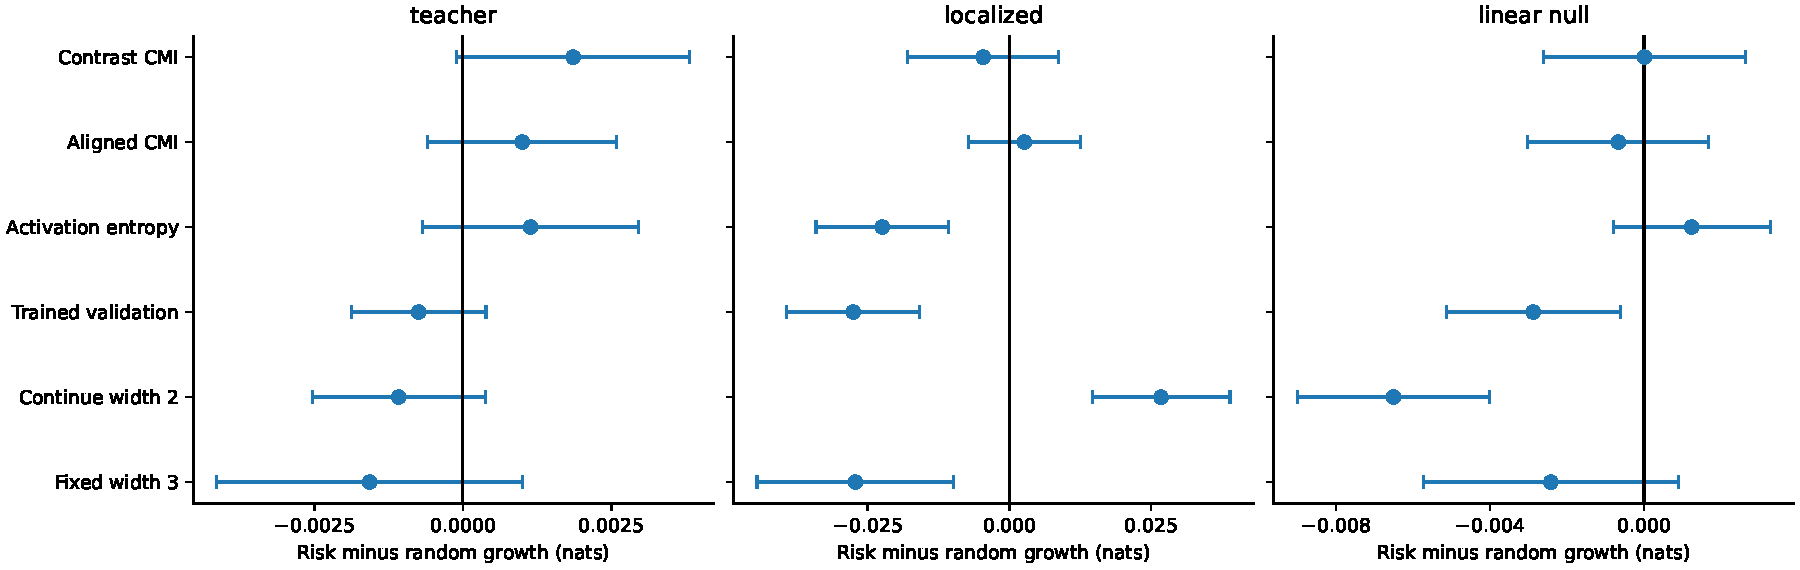
\includegraphics[width=\textwidth]{../figures/learning_information_aligned.pdf}
 \caption{Fresh-seed information-score ablation: paired risk differences from
 random growth over 32 independent repetitions, with 95\% Student-$t$ intervals.
 Aligned CMI uses the exact initial symmetric split logit deformation; contrast
 CMI uses the original antisymmetric activation contrast. Trained validation
 fits all eight candidates; fixed width 3 has a distinct initialization and a
 leading-width compute proxy. Risks average the true conditional label loss
 over 8192 held-out Gaussian inputs, not an exactly enumerated population.
 This plot is generated solely from saved experimental outputs.}
 \label{fig:aligned-information}
\end{figure}

The aligned score does not show a resolved advantage over random growth in
any of these three tests. Its paired mean differences are
$+0.000999\pm0.001588$ nats on the teacher task,
$+0.002634\pm0.009912$ on the localized task, and
$-0.000666\pm0.002350$ on the linear-null task, where each uncertainty is a
95\% Student-$t$ interval half-width across the 32 fresh seeds.
The localized task offers clear scope for improvement from additional capacity,
but the aligned information score does not identify the most useful operation:
its mean risk is $0.518572$, compared with $0.493478$ for the specified entropy
proxy and $0.488745$ for the fixed-width approximate-compute control.
The entropy proxy has a paired advantage over random growth of
$0.022459\pm0.011681$ nats on this task, whose interval excludes zero; this
positive measured finding is retained alongside the information-score nulls.
This observation does not make marginal activation entropy a valid invariant
principle. It shows that, in this experiment, the proposed label-information
proxy failed even to outperform a simple competing score.

On the linear-null task, continuing width two achieves mean risk $0.529499$,
below the aligned-growth risk $0.535339$. Information-score selection in this
study was forced to grow and therefore did not itself solve the decision of
whether to grow. Trained validation often improves candidate selection, but it
pays to fit all candidates and is not evidence for a cheap information-based
controller. The original 32-seed antisymmetric-proxy run is also preserved:
its apparent four-seed localized-task benefit did not become a resolved
conditional-information advantage after expansion. The audit-triggered aligned
ablation prevents that initially flawed proxy from carrying the conclusion.

The supported advance is consequently narrow and explicit. Input--residual
geometry can identify a beneficial real neuronal operation from finite samples
at a constructed stationary checkpoint, whereas unit-local scalar observables
cannot identify its direction. Equal-capacity neural training verifies that
this matters under a short optimization budget. Longer training, ordinary
pretraining, irrelevant inputs, and no-signal tasks expose its limitations.
The information-score experiments further show that defining and estimating a
conditional label-information quantity does not by itself supply an effective
neural structural controller. These findings establish a testable bridge and
its failure boundaries, not a general autonomous architecture-learning method.

All raw runs, failed or unfavorable conditions, seed ranges, learned matrices,
model parameters, resource proxies, and rerunnable figure scripts are included.
The main neural studies use only the existing local NumPy/SciPy environment;
no GPU, cloud resource, paid API, external dataset, or system-wide installation
was used. The experiments contain one structural decision per run and do not
establish the behavior of repeated, lifelong growth.
